%
% This is a borrowed LaTeX template file for lecture notes for CS267,
% Applications of Parallel Computing, UCBerkeley EECS Department.
% Now being used for CMU's 10704 Spring 2015 Information Processing and
% Learning course taught by Aarti Singh and Akshay Krishnamurthy.  When
% preparing LaTeX notes for this class, please use this template.
%
% To familiarize yourself with this template, the body contains
% some examples of its use.  Look them over.  Then you can
% run LaTeX on this file.  After you have LaTeXed this file then
% you can look over the result either by printing it out with
% dvips or using xdvi. "pdflatex template.tex" should also work.
%

\documentclass[twoside]{article}
\setlength{\oddsidemargin}{0.25 in}
\setlength{\evensidemargin}{-0.25 in}
\setlength{\topmargin}{-0.6 in}
\setlength{\textwidth}{6.5 in}
\setlength{\textheight}{8.5 in}
\setlength{\headsep}{0.75 in}
\setlength{\parindent}{0 in}
\setlength{\parskip}{0.1 in}

%
% ADD PACKAGES here:
%

\usepackage{amsmath,amsfonts,graphicx}
\usepackage{hyperref}
\usepackage{enumerate}

%
% The following commands set up the lecnum (lecture number)
% counter and make various numbering schemes work relative
% to the lecture number.
%
\newcounter{lecnum}
\renewcommand{\thepage}{\thelecnum-\arabic{page}}
\renewcommand{\thesection}{\thelecnum.\arabic{section}}
\renewcommand{\theequation}{\thelecnum.\arabic{equation}}
\renewcommand{\thefigure}{\thelecnum.\arabic{figure}}
\renewcommand{\thetable}{\thelecnum.\arabic{table}}

%
% The following macro is used to generate the header.
%
\newcommand{\lecture}[4]{
   \pagestyle{myheadings}
   \thispagestyle{plain}
   \newpage
   \setcounter{lecnum}{#1}
   \setcounter{page}{1}
   \noindent
   \begin{center}
   \framebox{
      \vbox{\vspace{2mm}
    \hbox to 6.28in { {\bf 10-704: Information Processing and Learning
	\hfill Spring 2015} }
       \vspace{4mm}
       \hbox to 6.28in { {\Large \hfill Lecture #1: #2  \hfill} }
       \vspace{2mm}
       \hbox to 6.28in { {\it Lecturer: #3 \hfill Scribe: #4} }
      \vspace{2mm}}
   }
   \end{center}
   \markboth{Lecture #1: #2}{Lecture #1: #2}

   {\bf Note}: {\it LaTeX template courtesy of UC Berkeley EECS dept.}

   {\bf Disclaimer}: {\it These notes have not been subjected to the
   usual scrutiny reserved for formal publications.  They may be distributed
   outside this class only with the permission of the Instructor.}
   \vspace*{-4mm}
}
%
% Convention for citations is authors' initials followed by the year.
% For example, to cite a paper by Leighton and Maggs you would type
% \cite{LM89}, and to cite a paper by Strassen you would type \cite{S69}.
% (To avoid bibliography problems, for now we redefine the \cite command.)
% Also commands that create a suitable format for the reference list.
\renewcommand{\cite}[1]{[#1]}
\def\beginrefs{\begin{list}%
        {[\arabic{equation}]}{\usecounter{equation}
         \setlength{\leftmargin}{2.0truecm}\setlength{\labelsep}{0.4truecm}%
         \setlength{\labelwidth}{1.6truecm}}}
\def\endrefs{\end{list}}
\def\bibentry#1{\item[\hbox{[#1]}]}

%Use this command for a figure; it puts a figure in wherever you want it.
%usage: \fig{NUMBER}{SPACE-IN-INCHES}{CAPTION}
\newcommand{\fig}[3]{
			\vspace{#2}
			\begin{center}
			Figure \thelecnum.#1:~#3
			\end{center}
	}
% Use these for theorems, lemmas, proofs, etc.
\newtheorem{theorem}{Theorem}[lecnum]
\newtheorem{lemma}[theorem]{Lemma}
\newtheorem{proposition}[theorem]{Proposition}
\newtheorem{claim}[theorem]{Claim}
\newtheorem{corollary}[theorem]{Corollary}
\newtheorem{definition}[theorem]{Definition}
\newenvironment{proof}{{\bf Proof:}}{\hfill\rule{2mm}{2mm}}

% **** IF YOU WANT TO DEFINE ADDITIONAL MACROS FOR YOURSELF, PUT THEM HERE:

\newcommand\E{\mathbb{E}}       % Expectation
\newcommand\pr{\mathbb{P}}      % Probability
\newcommand\Exp{\mathcal{E}}    % Exponential Family
\renewcommand\L{\mathcal{L}}
\newcommand\Pds{\mathcal{P}}
\newcommand\R{\mathbb{R}}
\newcommand\X{\mathcal{X}}
\newcommand\Y{\mathcal{Y}}
\newcommand\e{\varepsilon}
\newcommand\sminus{\backslash}
\newcommand\nbr{\mathcal{N}}
\newcommand\qed{\qquad\ensuremath{\square}}
\renewcommand\hat{\widehat}
\newcommand\sgn{\operatorname{sign}}

\begin{document}
%FILL IN THE RIGHT INFO.
%\lecture{**LECTURE-NUMBER**}{**DATE**}{**LECTURER**}{**SCRIBE**}
\lecture{17}{March 24}{Aarti Singh}{Shashank Singh}

% **** YOUR NOTES GO HERE:

% Some general latex examples and examples making use of the
% macros follow.  
%**** IN GENERAL, BE BRIEF. LONG SCRIBE NOTES, NO MATTER HOW WELL WRITTEN,
%**** ARE NEVER READ BY ANYBODY.

\section{Overview}

In the previous lecture we defined Sufficient Statistics, which capture all
information in the data relevant to estimating a desired parameter (hopefully,
in a concise way). Motivated by the fact that useful sufficient statistics
(i.e., those with dimension independent of sample size) only exist for certain
(i.e., exponential family) distributions, we defined two more general notions,
the Rate Distortion Function and the Information Bottleneck Principle.

In this lecture, we begin by introducing Channel Coding, a fundamental problem
in Information Theory, and presenting the Channel Coding Theorem. We then
review the rate distortion function, including the Rate Distortion Theorem,
and the Information Bottleneck Method and relate these to Channel Coding.

\section{Channel Coding}
\subsection{Introduction and Setup}
Recall that, in the source coding problem, we had the following model of
infomation flow:
\[\mbox{Source $\stackrel{W_1^M}{\xrightarrow{\hspace*{1.2cm}}}$ Source Encoder
$\stackrel{X_1^n}{\xrightarrow{\hspace*{1.2cm}}}$ Source Decoder
$\stackrel{\hat W_1^M}{\xrightarrow{\hspace*{1.2cm}}}$ Receiver}.\]
In particular, the decoder received exactly the stream emitted by the encoder,
and, given an input distribution $p(X_1^n)$, we were interested in designing a
conditional distribution $p(X_1^n | W_1^M)$ minimizing the expected length $n$
of the code (or, more precisely, the limiting ratio $\frac{n}{m}$ as
$m \to \infty$).

In the channel coding, we are again given an input string $W_1^n$ which we may
encode as $X_1^n$ we wish. This time, however, noise in introduced into $X_1^n$
(according to a known noise distribution), to create a new string $Y_1^{n'}$,
and then $Y_1^{n'}$ is given to the decoder, as shown below:
\[\mbox{Source $\stackrel{W_1^M}{\xrightarrow{\hspace*{1cm}}}$ Channel Encoder
$\stackrel{X_1^n}{\xrightarrow{\hspace*{1cm}}}$ Channel
$\stackrel{Y_1^n}{\xrightarrow{\hspace*{1cm}}}$ Channel Decoder
$\stackrel{\hat W_1^M}{\xrightarrow{\hspace*{1cm}}}$ Receiver}.\]
We will focus on discrete, memoryless channels, where this noise can be encoded
as a (known) conditional distribution $p(y|x)$ (i.e., each symbol $X_i$ is
mapped to $Y_i$ according to a fixed distribution, so $n' = n$). The goal is
then to design an encoding in the form of a distribution $p(x)$ that
(asymptotically) achieves low probability of decoding errors
$\frac{1}{M} \sum \pr\left[ \hat W_i \neq W_i \right]$, while again minimizing
the length $n$ of the code (or, more precisely, maximizing the rate
$\frac{M}{n}$ as $M \to \infty$). The main result, due to Shannon in 1948
\cite{S48}, is
the Channel Coding Theorem (also known as Shannon's Theorem), which identifies
the rates of codes that can achieve low decoding error in terms of the mutual
information $I(X;Y)$.

\subsection{The Channel Coding Theorem}
{\bf Definition:} The \emph{capacity} $C$ of a channel with noise distribution
$p(y|x)$ is defined as $C := \max_{p(x)} I(X;Y)$

{\bf Example (Binary Symmetric Channel)} The binary symmetric channel $BSC(p)$
parametrized by $p \in [0,1]$ has the noise distribution
\[P(y | x)
    = \left\{
            \begin{array}{ll}
                p & y \neq x    \\
                1 - p & y = x
            \end{array}
        \right.,
\quad \mbox{ for all } x,y \in \{0,1\}.\]
That is, $BSC(p)$ flips the input bit with probability $p$, as illustrated in
Figure \ref{fig:BSC}.
\begin{figure}[h!]
\centering
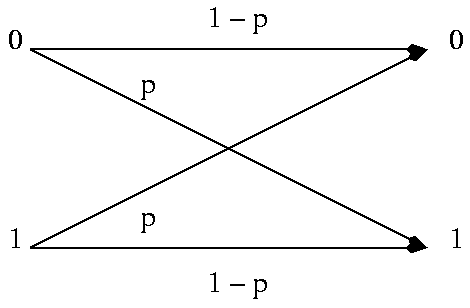
\includegraphics[width=0.35\textwidth]{BSC}
\caption{A binary symmetric channel with error probability $p$.}
\label{fig:BSC}
\end{figure}

For any input distribution $P(x)$, for $X \sim P(x)$ and $Y \sim P(y|X)$,
\begin{equation}
I(X; Y)
    = H*Y) - H(Y | X)
    = H(Y) - h(p)
    \leq 1 - h(p).
\label{ineq:BSC_cap}
\end{equation}
where $h(p) = -p \log p - (1 - p) \log(1 - p)$ is the entropy of
$\mbox{Bernoulli}(p)$. Furthermore, if $X \sim \mbox{Bernoulli}(\frac12)$, then
by symmetry, then $Y \sim \mbox{Bernoulli}(\frac12)$, and so $H(y) = 1$. Thus,
equality holds in (\ref{ineq:BSC_cap}), and so the capacity of $BSC(p)$ is
$C_{BSC(p)} = 1 - h(p)$. \qed

{\bf Definition:} Consider a discrete, memoryless channel. A rate $R$ is called
\emph{achievable} iff there exists a $(2^{nR}, n)$-channel code with
asymptotically vanishing error, i.e.,
\[\lim_{M \to \infty}
    \frac{1}{M} \sum_{i = 1}^M \pr\left[ \hat W_i \neq W_i \right] = 0.\]

{\bf Theorem (Channel Coding):} A rate $R$ is achievable if
$R < C := \max_{p(x)} I(X;Y)$, and unachievable if $R > C$.

Here, we will prove only the ``if'' statement (i.e., \emph{achievability}).
Later in the course, we will prove the ``only if'' statement (i.e.,
\emph{necessity}), which will be useful for proving lower bounds in machine
learning problems.

Like the proof of achievability for the source
coding theorem, the proof here uses a simple (albeit, impractical) coding
scheme based on the notion of \emph{typicality}. Rather than just typicality of
the input stream $X_1^n$, however, we require a stronger condition:
\emph{joint typicality} of the joint input and output stream $(X_1^n,Y_1^n)$.

\newpage
{\bf Definition:} Given a joint probability density $p : \X \times \Y \to R$
with marginal densities $p_X$ and $p_Y$, the \emph{jointly typical set}
$A_\e^{(n)} \subseteq \left( \X \times \Y \right)^n$ is the set of sequences
$\{(x_i,y_i)\}_{i = 1}^n \in \left( \X \times \Y \right)^n$ such that
\begin{enumerate}
\item $\left| -\frac{1}{n} \sum_{i = 1}^n \log p_X(x_i) - H(p_X)\right| < \e$,
\item $\left| -\frac{1}{n} \sum_{i = 1}^n \log p_Y(y_i) - H(p_Y)\right| < \e$,
\item $\left| -\frac{1}{n} \sum_{i = 1}^n \log p(x_i,y_i) - H(p)\right| < \e$.
\end{enumerate}

{\bf Theorem (Joint AEP):} The jointly typical set $A_\e^{(n)}$ satisfies
\begin{enumerate}[1)]
\item For $\{(x_i,y_i)\}_{i = 1}^n$ drawn i.i.d. from $p$,
\[\lim_{n \to \infty} \pr[\{(x_i,y_i)\}_{i = 1}^n \in A_\e^{(n)}] \to 1.\]
\item $|A_\e^{(n)}| \leq 2^{n(H(X,Y) + \e)}$
\item for sequences $\tilde x_1,\dots,\tilde x_n \sim p_X$ and
$\tilde y_1,\dots,\tilde y_n \sim p_Y$ drawn independently,
\[\pr\left[ \{(\tilde x_i,\tilde y_i)\}_{i = 1}^n \in A_\e^{(n)} \right]
    \leq 2^{-n(I(X;Y) - 3\e}.\]
\end{enumerate}

\emph{Proof:} Property 1) follows from the Weak Law of Large Numbers and a
union bound. Property 2) follows from the basic AEP (which we proved with the
source coding theorem). Property 3) follows from property 2) and parts 1. and
2. of the definition of $A_\e^{(n)}$ because
\begin{align*}
\pr\left[ \{(\tilde x_i, \tilde y_i)\}_{i = 1}^n \in A_\e^{(n)} \right]
 &  = \sum_{\{(x_i,y_i)\}_{i = 1}^n \in A_\e^{(n)}}
                                            \prod_{i = 1}^n p_X(x_i)p_Y(y_i) \\
 &  \leq 2^{n(H(X;Y) + \e)}2^{-n(H(X) - \e)}2^{-n(H(Y) - \e)}
    = 2^{-n(I(X;Y) - 3\e},
\end{align*}

\emph{Proof (Achievability of Channel Coding):} Suppose $R < C$.
\emph{Coding Scheme:}
The encoder and decoder operate as follows:
\begin{enumerate}
\item Generate $2^{nR}$ i.i.d. codewords of length $n$ according to the
distribution
\[p(x_1^n) = \prod_{i = 1}^n p(x_i).\]
These strings form the (ordered) codebook $\mathcal{C}$, which is known to both
the encoder and the decoder. For $W \in \{1,\dots,2^{nR}\}$, we write
$X_1^n(W)$ to denote the $W^{th}$ codeword in $\mathcal{C}$.
\item A length $nR$ binary message $W$ is generated uniformly at random (so
each $\pr\left[ W = w \right] = 2^{-nR}$).
\item The encoder transmits the codeword $X_1^n(W)$.
\item The decoder receives a noisy codeword $Y_1^n$ from the channel.
\item The decoder outputs an estimated message $\hat W \in \{1,\dots,2^{nR}\}$
if $\hat W$ is the \emph{unique} message with
$(X_1^n(\hat W), Y_1^n) \in A_\e^{(n)}$. If
$(X_1^n(\hat W), Y_1^n) \not\in A_\e^{(n)}$ or another
$\hat W' \in \{1,\dots,2^{nR}\}$ also satisfies
$(X_1^n(\hat W'), Y_1^n) \in A_\e^{(n)}$, the decoder outputs $\hat W = 0$
(i.e., it reports failure).
\end{enumerate}

\emph{Analysis:}
If we send $M$ messages independently as described above, then
\[\frac{1}{nR} \sum_{i = 1}^{nR} \pr\left[ W_i \neq \hat W_i \right]
    = \pr\left[ W \neq \hat W \right]
    = \pr\left[ (X_1^n(W),Y_1^n) \notin A_\e^{(n)} \right]
    + \pr\left[ \exists \hat W' \neq \hat W
                \mbox{ with } (X_1^n(\hat W'), Y_1^n) \in A_\e^{(n)} \right].
\]
Part 1) of the joint AEP implies that that the first probability vanishes as
$n \to \infty$. For $\hat W' \neq \hat W$, $X_1^n(\hat W')$
was generated independently of $X_1^n(\hat W)$ from $p$ (and hence
independently of $Y_1^n$). Thus, applying a union bound, part 3) of the joint
AEP implies, for $\e = \frac{I(X;Y) - R}{6} > 0$,
\begin{align*}
\pr\left[ \exists \hat W' \neq \hat W
                \mbox{ with } (X_1^n(\hat W'), Y_1^n) \in A_\e^{(n)} \right]
    \leq \sum_{\hat W' \neq \hat W} \pr\left[ (X_1^n(\hat W'),Y_1^n) \in A_\e^{(n)} \right]
    \leq 2^{nR} 2^{-n(I(X;Y) - 3\e)}
    \to 0,
\end{align*}
as $n \to \infty$, proving the theorem.

\section{The Rate-Distortion Theorem}

Recall that the Rate Distortion function is
\begin{equation}
R(D) := \inf_{p(t|x)} I(X;T)
            \quad \mbox{ subject to } \quad \E\left[ d(X,T) \right] \leq D.
\label{eq:rate_dist_func}
\end{equation}

In practice, while we can't typically compute the rate distortion function
$R(D)$, we can approximate it via the Blahut-Arimoto algorithm (\cite{A72} and
\cite{B72}). This doesn't, however, give the optimal code.

{\bf Definition:} A rate-distortion pair $(R,D)$ is achievable if and only if
there exists a $(2^{nR},n)$ code with
\[\lim_{n \to \infty} \E\left[ d(X_1^n,\hat X_1^n) \right] \leq D.\]

{\bf Theorem (Rate-Distortion):} The rate-distortion function $R(D)$ defined in
(\ref{eq:rate_dist_func}) gives the maximum achievable rate at distortion level
$D$.

The proof of the rate-distortion theorem is similar to the proof of the channel
coding theorem. The main addition is that the typical set needs one addtional
property: \emph{distortion typicality}. In particular, we add the condition
$|d(x_1^n, \hat x_1^n) - \E\left[ d(X_1^n, \hat X_1^n) \right] \leq \e$ in
order for $(x_1^n, \hat x_1^n)$ to be in $A_\e^{(n)}$.

{\bf Example (Compressing Gaussians):} Suppose $X \sim
\mathcal{N}(0,\sigma^2)$ (where $\sigma$ is known) and $d(x,t) = (x - t)^2$.
Then, the rate distortion function is
\[R(D) = \left\{
            \begin{array}{ll}
                \frac{1}{2} \log \left( \frac{\sigma^2}{D} \right)
                                            & \mbox{ if } D \in (0,\sigma^2) \\
                0 & \mbox{ else }
            \end{array}
    \right..
\]
When $D \in (0,\sigma^2)$, we can solve for the distortion in terms of the
rate: $D(R) = \sigma^2 2^{-2R}$. Suppose, we use a simple statistic
\[T = \left\{
        \begin{array}{ll}
            \E[X | X \geq 0] & \mbox{ if } X \geq 0 \\
            \E[X | X < 0] & \mbox{ else }
        \end{array}
    \right..\]
A straightforward computation gives
$\E[X | X \geq 0] = \sqrt{\frac{2}{\pi}}\sigma$, and, symmetrically,
$\E[X | X < 0] = -\sqrt{\frac{2}{\pi}}\sigma$, so $T =
\sgn(X)\sqrt{\frac{2}{\pi}}\sigma$.
$T$ can be transmitted using a single bit, and so, according to the
rate-distortion theorem, the optimal distortion is $\frac{\sigma^2}{4}$. On the
other hand, while $T$ appears to be an optimal $1$-bit compression of $X$,
\begin{align*}
\E[(X - T)^2]
    = 2\int_0^\infty \left( x - \sqrt{\frac{2}{\pi}}\sigma \right)^2 \phi(x) \, dx
 &  = 2\int_0^\infty \left( x^2 - 2x\sqrt{\frac{2}{\pi}}\sigma + \frac{2}{\pi}\sigma^2 \right) \phi(x) \, dx    \\
 &  = \sigma^2 + \frac{2\sigma^2}{\pi} - \frac{4\sigma^2}{\pi}
    = \sigma^2 \left( \frac{\pi - 2}{\pi} \right)
    \approx 0.36 \sigma^2 > 0.25\sigma^2.
\end{align*}
Thus, the distortion is significantly ($44\%$ per symbol) higher than optimal.
The intuition is that the rate-distorition theorem is an asymptotic result;
by transmitting $T$ once per input $X$, we waste fractional bits that could be
used to reduce the average distortion if we encoded long input sequences with a
block code.

\section{Information Bottleneck Method}
The information bottleneck method tries to find a statistic $T$ that shares
minimal information with the data $X$, while still conveying information about
a parameter $Y$. It does so by finding a distribution over $T$, depending on
$X$, which minimizes the following criterion:
\[\min_{p(t|x)} I(X;T) - \beta I(T;Y),\]
where $\beta > 0$ is a Lagrange multiplier. It can be shown that the
rate-distortion problem is a special case of the information bottleneck
problem. This provides an intuitive link between the problems of channel coding
and of finding sufficient statistics.

\section{Continuous Channels}
We now briefly consider the case of a channel operating over an uncountable
alphabet. Suppose the channel takes input $X$ outputs $Y = X + \e$, where
$\e \sim \mathcal{N}(0,\sigma^2)$ is independent of $X$. In general, by
choosing the distribution of $X$ appropriately, we can make $I(X; Y)$
arbitrarily large. For example, if $X \sim \mathcal{N}(0,\eta^2)$, then
\[I(X;Y) = H(Y) - H(Y | X)
    = \frac{1}{2} \log\left( 2\pi e(\sigma^2 + \eta^2) \right)
    - \frac{1}{2} \log\left( 2\pi e(\sigma^2) \right)
    = \frac{1}{2} \log\left( \frac{\sigma^2 + \eta^2}{\sigma^2} \right)
    \to \infty
\]
as $\eta \to \infty$. Thus, the usual definition of channel capacity is
meaningless. A practical solution is to introduce a \emph{power constraint} of
the form $\E[X^2] \leq P$. From the maximum entropy property of the Gaussian
distribution, it is easy to see that the capacity of the above channel is then
$\frac{1}{2} \log\left( \frac{\sigma^2 + P}{\sigma^2} \right)$.

Next time, we will discuss continuous channels further, including applications
to areas such as privacy.

\section*{References}
\beginrefs
\bibentry{S48}{\sc C.E.~Shannon}, ``A Mathematical Theory of Communication.''
\underline{Bell System Technical Journal}, 1948.
\bibentry{A72}{\sc S.~Arimoto}, ``An Algorithm for Computing the Capacity of
Arbitrary DMCs'', \underline{IEEE Trans. I.T.}, pp. 14-20, Jan. 1972.
\bibentry{B72}{\sc R.~Blahut}, ``Computation of Channel Capacity and Rate
Distortion Functions'', \underline{IEEE Trans. I.T.}, pp. 460-473, July 1972.
% \bibentry{KB07}{\sc M.~Kalisch} and {\sc P.~B\"uhlmann}, 
% ``Estimating High-Dimensional Directed Acyclic Graphs with the PC-Algorithm,''
% {\it Journal of Machine Learning Research 8}, 2007, pp.~613--636.
\endrefs

\end{document}
